\documentclass[aspectratio=169,11pt]{beamer}

\usetheme{Madrid}
\usecolortheme{default}
\usefonttheme{professionalfonts}
\setbeamertemplate{navigation symbols}{}
\setbeamertemplate{footline}[frame number]

\usepackage{amsmath, amssymb, booktabs, graphicx}
\graphicspath{{../../assets/figures/}{assets/figures/}}

\title{Public Policy Targeting Workers}
\subtitle{Labor I -- Week 11}
\author{Teaching deck draft}
\date{}

\begin{document}

\begin{frame}
  \titlepage
\end{frame}

\begin{frame}{Central question and why this is the capstone}
\begin{itemize}
    \item Week 11 asks how labor economists evaluate policies that primarily act on workers rather than directly on firms.
    \item This is the worker-side capstone because it synthesizes incentives, dynamics, human capital, households, mobility, and frictions.
    \item The core challenge is to separate statutory policy from effective policy exposure.
\end{itemize}
\end{frame}

\begin{frame}{Weeks 2--10 mapped into policy margins}
\begin{itemize}
    \item Week 2: taxes, credits, and extensive versus intensive labor supply.
    \item Week 3: benefit timing, search incentives, and continuation values.
    \item Week 4: training and skill policy as dynamic investment.
    \item Week 6: childcare, leave, and household time allocation.
    \item Week 10: mobility support, search help, and place constraints.
\end{itemize}
\end{frame}

\begin{frame}{Unified framework}
\[
c_t = y_t + w_t h_t - T_t(w_t h_t, z_t) + e_t B_t(w_t h_t, z_t) - p_t^a a_t
\]

\begin{itemize}
    \item Policies act through incentives, constraints, insurance, frictions, and investment.
    \item Effective enrollment $e_t$ reminds us that eligibility is not treatment.
    \item The labor question is which worker-side margin actually moves.
\end{itemize}
\end{frame}

\begin{frame}{Policy channels and worker margins}
\begin{center}
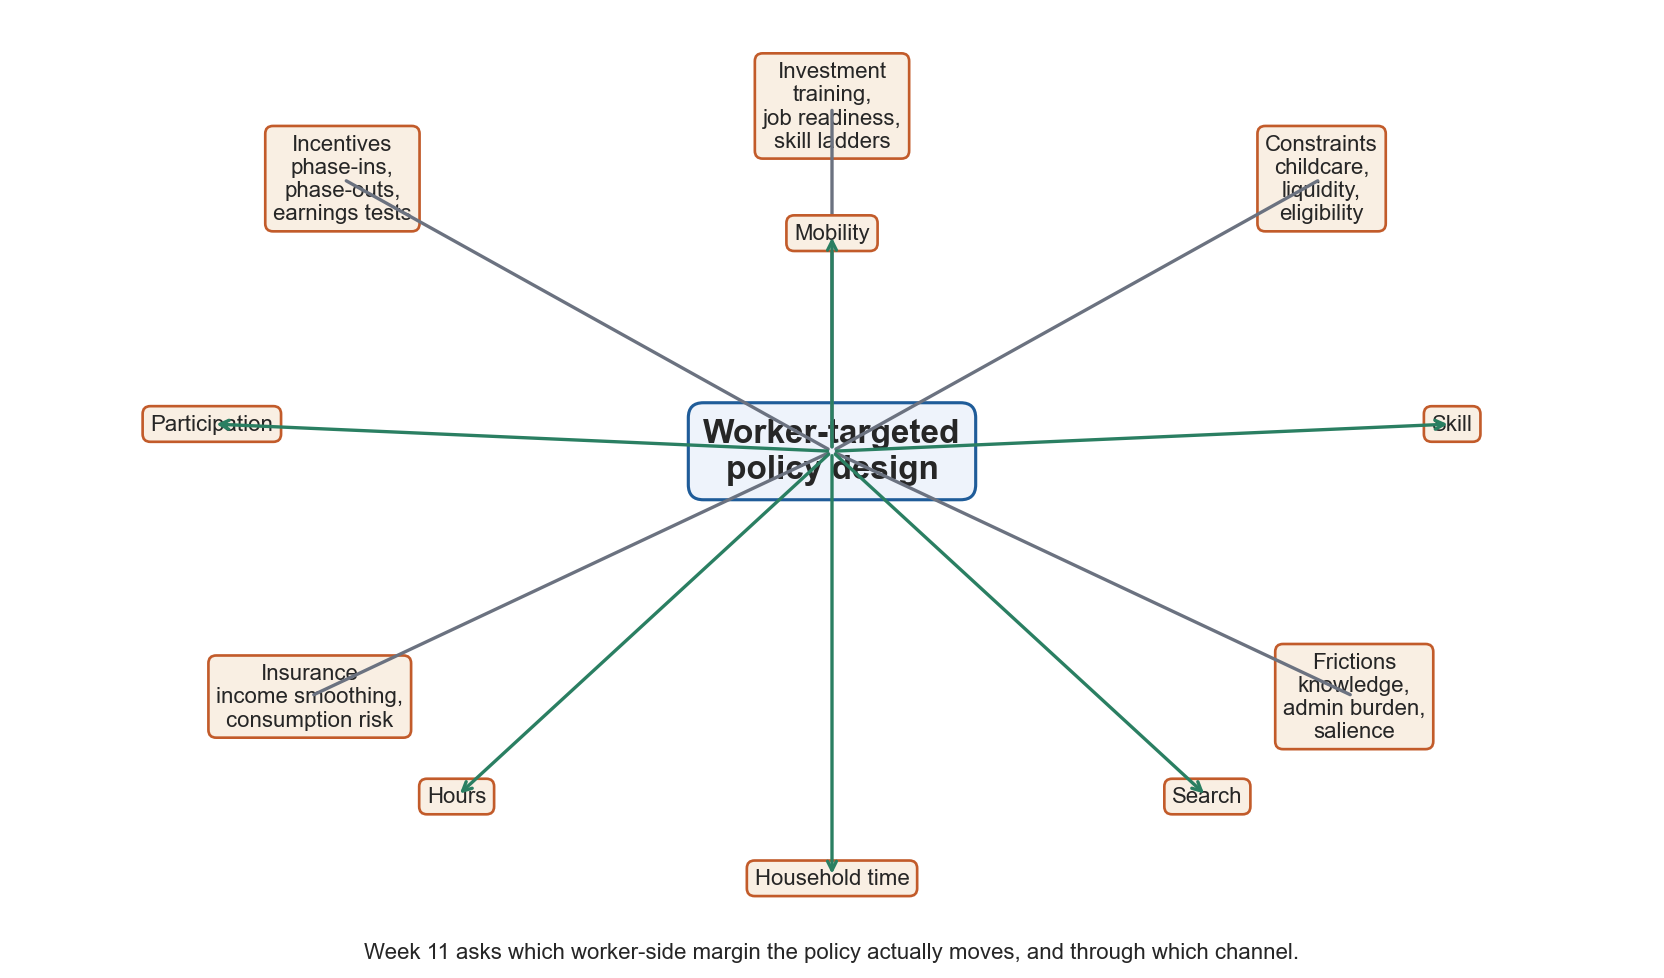
\includegraphics[height=0.72\textheight,keepaspectratio]{11-policy-margins-framework.png}
\end{center}
\end{frame}

\begin{frame}{EITC and in-work support}
\[
\frac{d \mathbb{E}[w h]}{d \theta}
= \bar{h} \frac{d \Pr(h>0)}{d \theta}
+ \Pr(h>0) \frac{d \mathbb{E}[h \mid h>0]}{d \theta}
\]

\begin{itemize}
    \item In-work credits often raise participation strongly while generating mixed hours responses.
    \item Phase-in, plateau, and phase-out regions imply different returns to earnings.
    \item Family structure matters for incidence and interpretation.
\end{itemize}
\end{frame}

\begin{frame}{Tax-credit schedule intuition}
\begin{center}
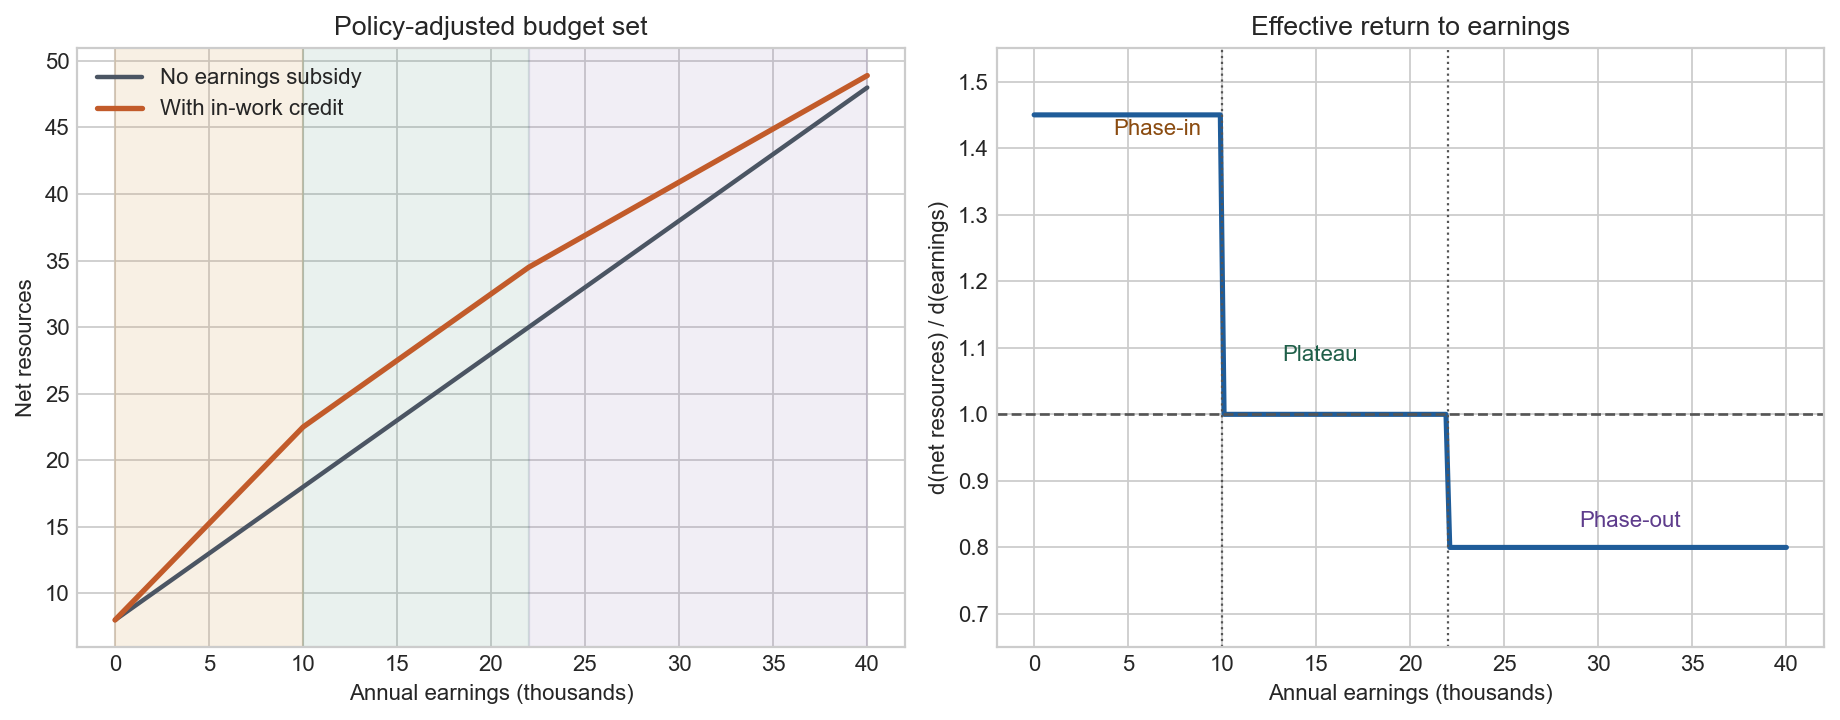
\includegraphics[height=0.72\textheight,keepaspectratio]{11-tax-credit-budget-set.png}
\end{center}
\end{frame}

\begin{frame}{UI, benefit timing, and search assistance}
\[
U_t(b_t) = u(c_t, \ell_t) + \beta \left[\lambda_t(b_t) W_{t+1} + \big(1-\lambda_t(b_t)\big) U_{t+1}(b_{t+1})\right]
\]

\begin{itemize}
    \item UI is an insurance object and an incentive object at the same time.
    \item Timing matters because liquidity needs are front-loaded over the unemployment spell.
    \item Search help can complement cash support rather than substitute for it.
\end{itemize}
\end{frame}

\begin{frame}{Training and skill policy}
\begin{itemize}
    \item Training should be evaluated dynamically, not only by short-run placement.
    \item Useful outcomes include earnings growth, occupational upgrading, and search quality.
    \item Job-readiness interventions often work through information and application quality.
\end{itemize}
\end{frame}

\begin{frame}{Family-support and time allocation}
\begin{itemize}
    \item Childcare and leave policy alter the shadow price of time inside households.
    \item Participation responses can be large even when hourly wage elasticities are modest.
    \item Household incidence matters: partner hours, bargaining, and care substitution may all move.
\end{itemize}
\end{frame}

\begin{frame}{Disability and retirement incentives}
\begin{itemize}
    \item Disability receipt is a labor-supply object and a household-insurance object.
    \item Retirement earnings tests and thresholds create dynamic incentives and local bunching opportunities.
    \item Judge or examiner assignment is often the key source of identifying variation.
\end{itemize}
\end{frame}

\begin{frame}{Take-up, salience, and administrative burden}
\[
D_i = \mathbf{1}\left\{\mathbb{E}_i[B_i \mid \mathcal{I}_i] - \kappa_i - \phi_i - s_i > 0\right\}
\]

\begin{itemize}
    \item Take-up is the bridge from statutory generosity to effective exposure.
    \item Null labor-market effects may reflect a weak delivery first stage rather than zero responsiveness.
    \item This is the direct bridge to Week 12 frictions.
\end{itemize}
\end{frame}

\begin{frame}{The take-up funnel}
\begin{center}
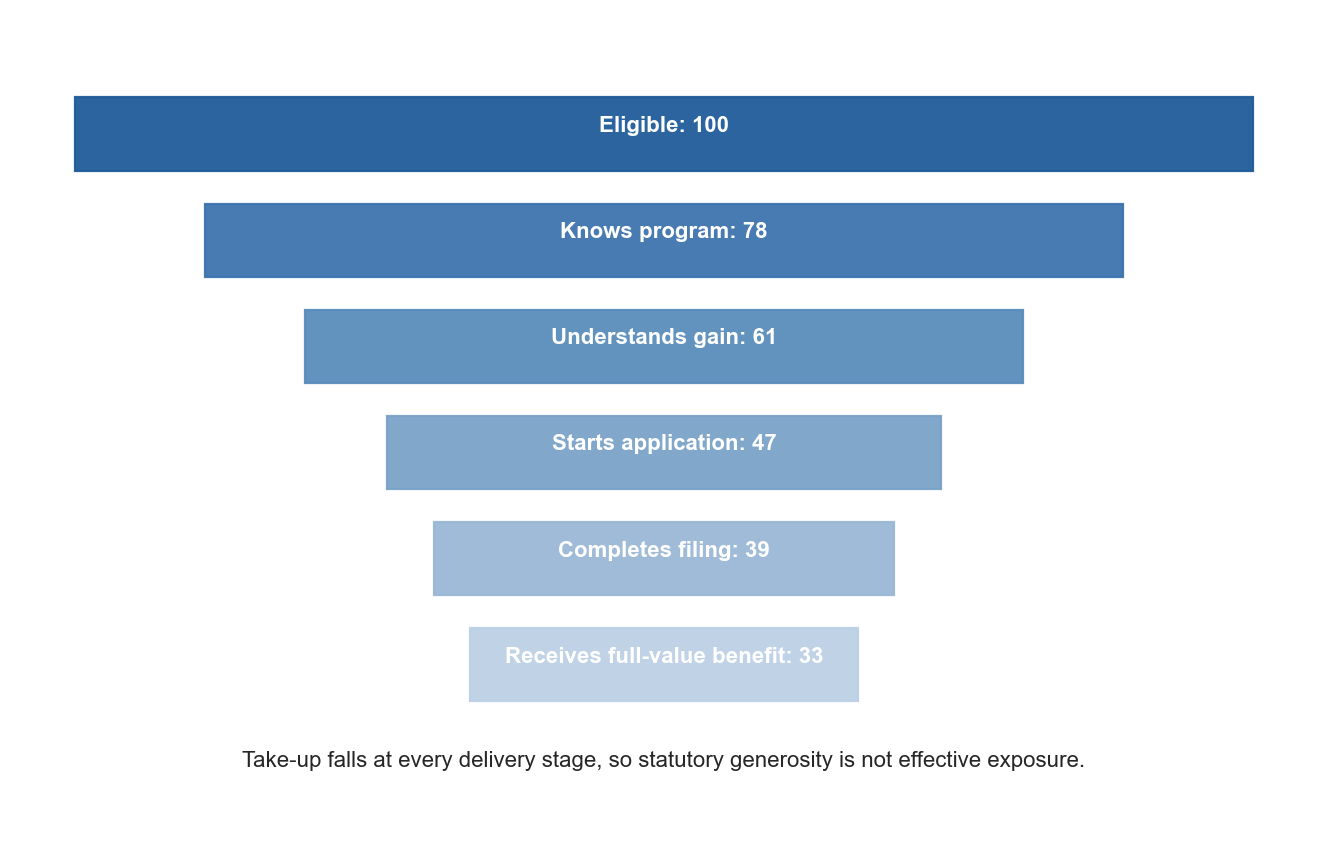
\includegraphics[height=0.72\textheight,keepaspectratio]{11-takeup-salience-funnel.png}
\end{center}
\end{frame}

\begin{frame}{Empirical design toolkit}
\[
\tau^{IV} = \frac{\operatorname{Cov}(Z_i, Y_i)}{\operatorname{Cov}(Z_i, D_i)}
\]

\begin{itemize}
    \item Kink and bunching designs match nonlinear schedules and thresholds.
    \item Field experiments and encouragement designs match delivered interventions and take-up.
    \item Reform event studies, judge IV, and knowledge-exposure designs match different institutions.
\end{itemize}
\end{frame}

\begin{frame}{Design choice must match the policy margin}
\begin{center}
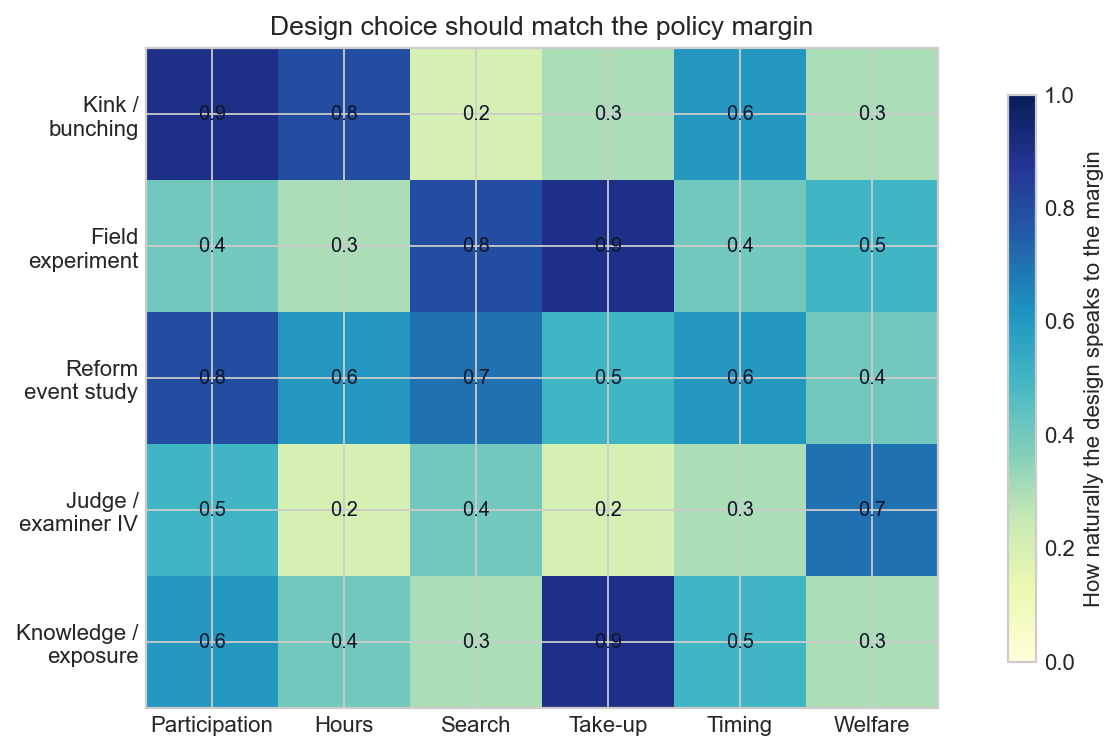
\includegraphics[height=0.72\textheight,keepaspectratio]{11-policy-design-toolkit.png}
\end{center}
\end{frame}

\begin{frame}{Welfare and design interpretation}
\[
\frac{dW}{d\theta}
=
\sum_i \omega_i \frac{\partial c_i}{\partial \theta}
- \lambda \sum_i \frac{\partial y_i}{\partial \theta}
+ \sum_i \eta_i \frac{\partial D_i}{\partial \theta}
\]

\begin{itemize}
    \item Employment effects are not enough for worker-policy ranking.
    \item Insurance, redistribution, delivery gains, and distortion costs all matter.
    \item Heterogeneity in constraints and frictions changes welfare ranking.
\end{itemize}
\end{frame}

\begin{frame}{Insurance-distortion frontier}
\begin{center}
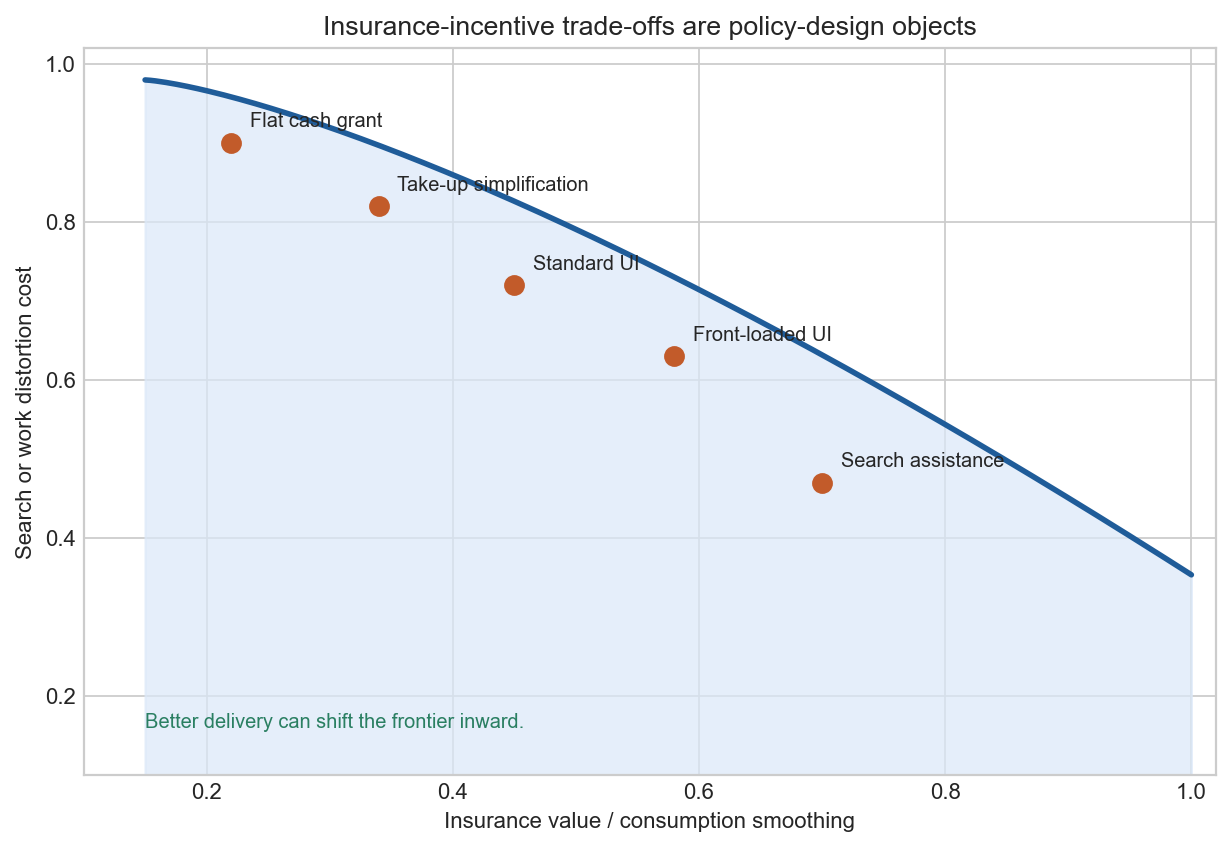
\includegraphics[height=0.72\textheight,keepaspectratio]{11-insurance-incentive-frontier.png}
\end{center}
\end{frame}

\begin{frame}{Researcher's checklist and bridge to Week 12}
\begin{itemize}
    \item What exactly is the policy object?
    \item Which worker-side margin is supposed to move?
    \item What frictions intervene between statute and exposure?
    \item What identifying variation matches the institutional margin?
    \item Which outcomes are dynamic, and what welfare claim is actually justified?
\end{itemize}
\end{frame}

\begin{frame}{Takeaways}
\begin{itemize}
    \item Worker-targeted policy is the place where Labor I theory and modern design meet.
    \item The same policy can work through incentives, insurance, or frictions.
    \item Take-up and administrative design are first-order labor objects.
    \item Week 12 begins where Week 11 ends: with labor supply under frictions.
\end{itemize}
\end{frame}

\appendix

\begin{frame}{Appendix: optional extension block}
\begin{itemize}
    \item Administrative burden and take-up.
    \item Front-loaded unemployment benefits.
    \item Household insurance and disability receipt.
\end{itemize}
\end{frame}

\end{document}
